\documentclass[conference,compsoc]{IEEEtran}
\ifCLASSOPTIONcompsoc
  \usepackage[nocompress]{cite}
\else
  \usepackage{cite}
\fi
\ifCLASSINFOpdf
\else
\fi

\usepackage{listings}

\usepackage{graphicx}
\graphicspath{ {images/} }

\begin{document}
\title{Final Report}

\author{\IEEEauthorblockN{Hugo Genesse}
\IEEEauthorblockA{Computer Engineering\\
Polytechnique Montreal\\
Montreal, Quebec\\
hugo.genesse@polymtl.ca}}

\maketitle
\begin{abstract}
MemSan's initial goal was to become a user-supplied data flow analyzer targeting memory-sensitize functions like strcpy that could lead to buffer overflow vulnerabilities. This paper will explain the steps that succeeded and those that didn't, the architecture, the problems encountered and some ideas on how the process could have been improved.
\end{abstract}

\IEEEpeerreviewmaketitle



\section{Introduction}
% no \IEEEPARstart

The project was split up into 5 parts: metrics extraction, UML class diagrams construction, Control Flow Graph extraction, dominator analysis and, 
finally, program slicing. Four of the five steps were done and can work on some more trivial examples that do not require a complex compilation process
 with multiple dependencies and modern C++ constructs like multiple namespaces. One problem that will be discussed is the fact that some of the last steps
 are dependant on each other and a problem on the CFG might impact the development speed drastically.

\section{Testing}
The project can be compiled with the provided Makefile and outputs the LOG6302 binary.
 There is also a "analysis" Makefile target that can be triggered to run the python script that will output the
 different .dot files and one target especially for the first lab that can be triggered with the "-tp1" switch on the Analyzer.py script 
.csv for the metrics for with the "tp1" target in the Makefile.

\section{Metrics extraction}
\subsection{Introduction}
The first part was metrics extraction like the number of if statements and method and class name. The relevant piece of code is in the src/metrics.py file and the parseClass function.
\subsection{Methodology}
 First, it is needed to reconstruct a simplified AST that will be processed later. We produce our own AST representation because our tool is aimed at specific goals and would be obstructed by the number of attributes the original clang AST. We are then decoupled from clang and can more easily implement new parsers and use the same code for the same analysis. For example, our AST output for the same code fits in 20 lines of XML instead of 81 lines of a the custom clang AST output format with also has longer lines. As you can also see, we have full control of our format to ease our post processing.
At that step, our custom AST was simple, without any metadata needed for other analyses and consisted only of basic blocs like while statetements, for statements, if's and variables.
\subsubsection{Custom AST implementation}
Using clang's RecursiveASTVisitor, some methods were overriden to
 redefine the behaviour the visitor on specific elements that I
 wanted to analyze. I then redefined 5 different traverses and 2 visits.
The redefined traverses are the following: TraverseWhileStmt, TraverseIfStmt,
TraverseCXXMethodDecl, TraverseCXXRecordDecl, TraverseFunctionDecl. We chose to
override traverses for those because they can encapsulate other elements I am
interested in and it is then important to visit its children. For example, a 
class will have methods definitions inside of it and I needed information on the
latter to complete our analysis. Because the other 2 elements, VarDecl and BreakStmt, are simpler elements that can't encapsulate others that I want to analyze, visits
sufficed to create opening and closing XML tags for our custom AST. The XML format 
was chosen for its wide use and tree-like structure that fits ASTs well. 
Elements were subsequently added in the other parts of the project.
\subsubsection{Metrics analysis}
The code metrics extraction is written in Python3 and entirely decoupled from clang. 
The metric extraction was then a simple walk of the resulting XML tree that counted each instance of code we wanted to measure.
The result is exactly what was provided in the project's description which means
 a CSV file with the following 
format: ID, FILENAME, CLASSNAME, METHODNAME, \#IF, \#WHILE, \#BREAK, \#VARS.
 It starts and finishes with a `dump` tag that 
encapsulates each files that were processed.

\subsection{Results}

The example used for the testing was the one provided, i.e. tests/LOG6302\_TP1\_example.cpp.
 It consists only of one method definition (function metrics were not calculated and
 therefore the main function is not analyzed) Bar in the Foo class. Metrics can be found in
 the src/metrics.txt file. For the provided example, we then have the following line for
 output :
\par
0, LOG6302\_TP1\_example.cpp ,Foo,bar,1,0,0,0
\par

This is the correct output because we have the correct filename, a unique ID,
 the correct class name, method name, and there is only one if instance, which was
 correctly calculated.
\subsubsection{Running the project}
To test these results, it is possible to re-run the LOG6302 on any method and
 run the Makefile with the tp1 target (make tp1).


\subsection{Difficulties}

\subsubsection{LLVM version}

Apart from getting the right version of llvm for the project, no real difficulty was encountered at this stage of the project.
 I tried the other llvm versions but couldn't make the seed project work with it. I think it would be best to update the seed
 project to the latest stable llvm version because that caused me some issues where the official documentation that is more 
 easily searchable with Google than its offline counterpart. Because the seed project was a couple versions late, some methods
 that would have been helpful in some cases and were explained in the online documentation was not in the 3.3 version.
 For example, many ways are used to get the line number in clang and some have been created in the last few versions which
 made those methods appear in the documentation but couldn't be used in the project.
\subsubsection{Backwards compatibility}

 For the final project, I think it wasn't
 clear that the final project needed to incorporate all the parts and be able to output every step to be evaluated as I thought
 that I was already submitted and reviewed so I worked on the previous version of my code base and deleted some functions and changed the way some things worked.
 This broke retro-compatibility but wsa fixed for the first lab but wasn't for the second as you will see.

\section{UML class diagrams}
\subsection{Introduction}

The second part of the project was to build UML class diagrams from
 C++ source code. This part took more time than the first lab but didn't
 prove itself a real problem like the CFG extraction was. I lacked time to
 properly add this part of the project to the final project and is then located
 in its own folder in MemSan/tp2 with its own build process. It is possible to test
 these functionalities in the tp2/ directory with the same process as the main project.
 The interesting code is in the several nodes created and the parseClass method of the Analyzer class.

\subsection{Methodology}

 \par For the UML class diagrams, I didn't need
 the number of local variables, break statements, if statements
 and while statements. I ended up initially deleting that part of the code and broke backwards compatibility like so.
 The code to generate the UML class diagrams is then in another folder by itself as a snapshot of the release of the
 second lab.
 Only one
 visit was added, the FieldDecl one. This one provides a visit
 for the class attributes. The type also needed to be extracted
 in our AST. Luckily, the getType() method was defined with the
 getAsString() method to convert from internal clang types to strings.
 This was used for CXXRecordDecl which are classes and FieldDecl.
 For methods, getResultType() was called to resolve the return value type.
 This one proved tricky as it will be explained in the difficulties section later.
 For the XML part, the following tags were added: parentClass that stores the
 name of the base class in case the class MemSan is analyzing inherits from another one,
 methodReturnType that stores the return value type of that method. Also, since the
 attributes were new in this part of the project, I needed tags to identify them.
 We added the attribute tag to encapsulate all the attributes information
 As I couldn't get a real project meeting the course requirements to compile using my
 tool, the test called LOG6302\_TP1\_example.cpp was heavily modified to test the new use
 cases. The new file is named LOG6302\_TP2\_example.cpp and is located in the tests folder. 
 I now use a base class named BaseClass that has one public and one private
 attribute and a method that returns a void*. One class inherits from this base class
 and is called ChildClass. The third and final class doesn't use inheritance but
 has an attribute that is of the type BaseClass. This example can then demonstrate
 most of the use cases.

\subsection{Results}

 Apart from the fact that all methods and attributes are private because no logic
 to verify that the method is public or private has been implemented. From the official
 documentation, the isPublic() method should be accessible to verify this quite easily
 but the 3.3 version doesn't seem to have such methods on the same types of objects which
 complicated that implementation. The results for the LOG6302\_TP2\_example.cpp file that
 can be found in the root folder of the tp2 subfolder are in appendix 2.

\subsection{Difficulties}
\subsubsection{Real project compilation}
 Some significant amount of time before the deadline of that part of the project was on trying
 to compile a big code base with more than 100K LOC. Various projects were tested to try to make it
 work like the code base of Firefox, chromium, chromium-os, kvm and sqlite. Sqlite was the most
 promising but, as it is C and not C++, it couldn't be used for the UML class diagram part of the
 project since C doesn't have the concepts of classes, inheritance and so on. Global namespaces
 were also a challenge and was fixed much later on with the use of only libcxx from llvm and not
 its GNU equivalent. This was only known a few days before the final deadline and then couldn't
 be used properly because other small bugs appeared during the parsing. After researching the final
 issues I had with the compilation of a major project, I found only one reference of this issue
 in the LLVM mailing list and was not resolved to this date. I then decided to focus on other parts
 of the project instead.

\section{CFG Extraction}
\subsection{Introduction}
This is the part where I had the most problems with. Because the next steps needed a perfect CFG.
 I needed to make sure my Control Flow Graph was good before I could be able to write more code or,
 because I implemented some parts of the code even when I still had a broken Control Flow Graph, be able
 to debug it correctly with the results making more sense. The interesting parts of the code are in the parse* functions
 in Analyzer as well as the recursiveDump and parseNode methods and the buildCFG and dump\_cfg methods.

\subsection{Methodology}
 Clang's ASTRecursiveVisitor was still used for the part
 that builds our own AST. Some parts were added like: VisitBreakStmt,
 VisitContinueStmt, VisitUnaryOperator, TraverseForStmt, TraverseReturnStmt.
 Python classes for the analysis part of the project
 were once again added to ease the analysis.
\subsubsection{Modifications introduced}

 Introduced in the second part of the project, Nodes were still used
 to interpret the output of the C++ part of the project. Although the core concept
 was the same (using nodes), a lot of refactoring had to take place to be able to walk
 the AST recursively as it eased the construction of the control flow graph. First,
 every node class was stripped down to only its name and then I added a node type to
 facilitate the implementation as I didn't need to check if the object was an instance
 of any node that could be possible. Every node was then added a children attribute
 that is a list of all its children. An edge will then be added between a parent node
 and a child node in the dumping process.
\subsubsection{Initial approach}
The walk of the AST is split into two catefories:
 one is responsible for the dispatch to the right parse function according to the XML tag
 that it reads so we don't have to repeat the dispatch code in every parse function of every
 node type. The second one are the parser functions which every node type has one of. Every
 node type has its own steps required like the WhileNode which needs a whileEnd and whileBegin
 as well as a testing condition to break out of the loop. Similar logic has been implement for
 the ForNode as well as the ifNode. The others are simpler and only need to be linked to its
 immediate predecessor as it is the case for the unaryOperator, ContinueStmt and BreakStmt. The
 ReturnStmt is a special case has it need to linked to the exit node. The exit node is a singleton
 node that is the first to be created to be able to link to it without errors when GraphViz parses
 the output of our tool.

\subsubsection{Problems with the first approach}
At first, the CFG produced was the one included in appendix 2. Some bugs were still present as you can see from the
figure. Firstly, the unaryOperator is in the wrong order as the returnStmt is currently a traverse
and the unaryOperator is treated like its child but it is the returnStmt that is linked to the
exit node. Secondly, some edges are missing and I couldn't find the bug in the logic in time.
 Thridly, some edges are duplicated as we can see in one of the return nodes. This is caused by the
 fact that the return node has multiple parents and causes the node to be visited multiple times and
 then the logic that is responsible for linking the return node to the exit nodes is executed
 multiple times.
\subsubsection{Issues explanation}
 Those issues can be explained with a few different reasons. First, the control
 structures like loops and conditional branches should have been completely structured
 as an independent block acting as any other node in the Control Flow Graph. I tried and
 was convinced that those should be linked in a more complicated fashion than it should have been.
 For example, the while node implementation has a condition node added to make the last statement of the inside
 of the loop 

\subsubsection{Revised approach}
 This previous methodology had problems and was tougher to debug and longer to implement because it
 needed to copy the changes made for the nodes on all nodes implementation which was a cause for some
 minor bugs. The final implementation was stripped down from all the possible code statements having
 a node class each, like ForNode for example, to one node implementation called BaseNode. This sped up
 the debugging but reduced overall code quality. At first, this was done to make a better visitor but,
 as method overriding is not possible as far as I can tell in Python3, this wasn't as useful as it
 wold have been in Java or C++ for example.

\subsection{Results}

The final results were a lot more convincing when the code was not as trivial as the initial tests were.
For example, the file results/final\_cfg.png shows the resulting CFG for the wc.c program. It was not included
 in this paper as it is much too big for the template. The only major bug that is still showing
 but doesn't affect the dominators analysis as much as other bugs that were more apparent in the structure is the fact
 that I didn't find a way to reliably see if the binaryOperators were used in the condition of a conditional statement
 or were inside the following statements. For example, a if statement is followed by a condition but the code inside the
 if statement can use binary operators like "<" and I did not want to match those as it was not a proper solution to the problem
 and that problem was not a real issue for the dominators analysis as only a few nodes were swapped. When the more complicated nodes
 such as loops and conditional statements were self-contained, I did not have problems with nonsensical edges that were added when
 those structures were embedded one inside the other.

\subsection{Difficulties}

 As the architecture is completely custom and really little amount of the course's notes are on the construction of the
 Control Flow Graph and how to handle some Control Flow statements like while and if can easily be translated to
 a structure that will fit a CFG correctly, some mistakes were made even in the conception phase of my Control Flow Graph
 because I took the Dragon's book approach for while statements, if statements and others but, conceptually, I had
 some issues with how it was represented when embedded in other constructs like whiles and ifs. For example, at first, it was close
 to working when the code was trivial but, even wc.c with ifs embedded in a while, my approach didn't work at all.

\section{Dominator Analysis}

\subsection{Introduction}
The next part that needed to be implemented was the analysis of the dominators in the program to be able to do
 control flow analysis. As this part of the project could have been as challenging as the previous one. A reference
 implementation was provided which helped a lot. The important code for this part are the java\_*dom\_tree and nca methods.

\subsection{Methodology and Results}
\subsubsection{Dominators}

The reference implementation was studied and reimplemented with my node structure in Python. For the dominators tree,
 the results that you can see in results/dom.png seem to be correct. The dominators are in one single tree and follow
 the logic of the definition of the dominators.

\subsubsection{Post-dominators}

I used the approach of reversing the parents and the children of all the nodes and running the dominators algorithm again
 to output the post-dominators but encountered a problem with my WhileEnd node which did not have a post-dominator tree parent
at the end of the algorithm and I still have not figured out why at the moment of the final release. As the next analysis are based on this result
 results will be affected and much harder to debug and verify their validity. The results for this analysis is provided in results/pdom.png.

\subsection{Difficulties}

 Because the dominators analysis and control dependency and so forth all relied on a correct CFG output,
 those bugs slowed me down dramatically and, frankly made me stressed and underwhelmed with the results.
 The problems with the post-dominator analysis and why it doesn't seem to affect the dominator analysis are still
 unknown. The hypothesis is that some incorrect children nodes are added for the while nodes and are not a problem
 for the dominator analysis but when switched with the parents for the post-dominators, it renders the end result wrong.
 The code that is responsible of adding those incorrect nodes was not found in time and therefore, the problem could not be fixed.

\section{Program Slicing}

\subsection{Introduction}
The final part of the project was to slice the wordcount program. A slice is defined as a subset of the code that is data and control independent from the rest.

\subsection{Methodology and Results}
\subsubsection{Control Dependency Graph}
After the post-dominator analysis, I tried to extract the Control Dependency Graph with the post-dominators tree.
I reimplemented the algorithm from the course slides the best I could. The final result is not really impressive but seems to show
 that the logic is partly right as the condition node that is working seems to have the correct nodes linked to it. The other nodes
are not working but seemed to be processed while debugging. The hypothesis is that a logic bug was introduced while implementing the
 verification of the post-dominance of one node compared to another that has an edge between the two. I tried swapping the logic but then
 caused an infinite loop.

\subsubsection{Data Dependency Graph}
For the data dependency graph, the clang logic was implemented in the sense that binary operators that were assignments were analyzed to extract
the left hand side to get the defined variable and the right hand side for the used variable. The left hand side was not hard to implement as it is easy to get the LHS from
a clang Expr but the right hand side was more difficult because it could consist of multiple variables or expressions like it is the case in the "nc = nc + 1" line in wordcount.
I looked for various ways to extract the right hand side variables but ended up writing the whole right hand side in the XML that would have been processed by the Python part later.
Due to a lack of time and results in the previous parts, the python processing and analysis of the valid references was not implemented.

\subsubsection{Linking everything together and output a slice}
As the previous two graphs were either wrong or not finished, the final slicing was not implemented.


\section{Final Results}
As I couldn't figure a way to make a real code base to compile. Real results could not be extracted and analyzed.


\section{General Difficulties}

\subsection{Real Project Compilation}
 I think this project required a major amount of time that was difficult to manage on a end of bachelors
 schedule. Before the Control Flow Graph, everything went smooth and required a decent amount of time.
 Also, as I really wanted to make a real project work, I spent some significant time on the problem while
 searching for the causes of those problems in a normal compiling context but the solutions didn't apply in my case
 as the code was supposed to compile without modification to the code but only the way it was loaded with the right
 dependencies and the correct flags. The solutions that were tried was to use the libcxx provided by llvm but I still
 had other includes that weren't compatible with my clang version which made me thought that the problem of dependencies
 couldn't be solved simply with the llvm libraries. I tried using older versions of libraries as my clang version was
 not up to date but this approach failed. Some projects, like chromium-os, copies a lot of its dependencies in the project
 to make changes to them and fix some problems without the need to wait for a patch of a third party. Those libraries were
 tested but I still had the same problems. Lastly, pre-processing of the code was tried but didn't solve all the problems as
 well and even created some. Pre-processing consisted of a small script that deleted the includes and namespace to solve those
 problems because undefined functions only caused warnings but deleting namespaces proved to be difficult to fix in big code bases
 that used them heavily like you would expect from a major modern C++ project.

\subsection{Time}
As many single point of failures could be encountered, the project stalled many times until debugging was done and code was corrected.
 This made me decide to double down on having complete features and some features missing instead of a big set of unfinished and incorrect features.
 Because the final steps of the project weren't finished and totally working, I prioritized the code to the quizzes which didn't help my understanding
 of the final steps and proved a bad choice.

\subsection{Control Flow structures}
As explained before, the problems I had with the Control Flow Graph took me a long time to fix properly and required
 some major changes in the project structure which impacted the final code quality, subsequent analyses based on the
 Control Flow Graph and made me loose some important amounts of time which were essential to the success of the project.

\subsection{Implementation bugs}
Some bugs were caused by Python more advanced features that I tried to leverage to make better and more compact code.
 One of the example is the comparison overloading with \_\_eq\_\_ methods on the BaseNode and Edge classes. This was useful to
 easily compare nodes and edges like they were standard types of the language but were hidden in other files while the big
 majority of the project's logic was in the Analyzer class. Since I had lots of problems with the Control Flow Graphs loops
 and conditional statements, it took me a while to find bugs that were related to those operations as they succeeded most of the time
 but failed in some edge cases like comparison with the FunctionNode which was a standalone node for functions that was a relic
 of the old project architecture. These also took time to debug and solve, which impacted the end result as well.

\subsection{Debugging}
 As the AST dumping logic was separated from the analyses, I had to go back and forth in two different parts of the project with distinct
 concepts related to each other. The XML output changed a few times and different bugs were introduced while making changes and were not as
 easy to see because the XML output was wrong but I thought that the analysis part was wrong. The output file was then more hidden and 
 tougher to see its problems when debugging in PyCharm.

\section{Conclusion}

I first thought the problems I had with the Control Flow Graph were trivial but needed a complete restructuration of my
 approach and even of the whole project's structure to ease the implementation, changes and debugging. I am not satisfied
 with the end result has it fails to reach the ultimate goal of program slicing and even data dependency. I think I should have spent
 more time before the fourth lab to fix my Control Flow Graph and ask questions and reach out for help before I was in trouble.
 I also think this a major single point of failure for the project and should be reviewed thoroughly to make sure students will
 be able to make progress in the following weeks. I also think an initial backup project should be provided to be guaranteed to work
 if the student chooses to use clang as it is the default seed project for the course.


\section{Appendix}
\subsection{UML class diagram}
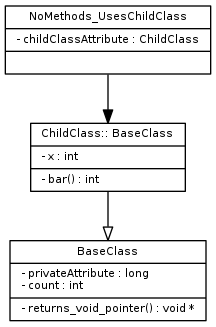
\includegraphics{uml}
\subsection{First release of the CFG}
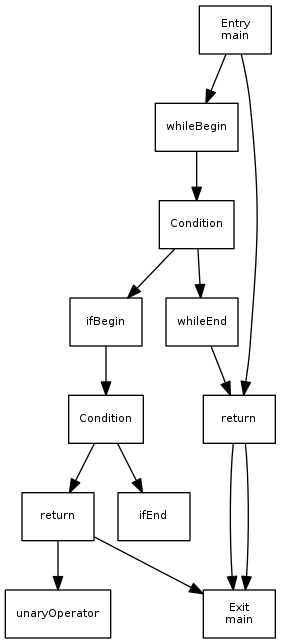
\includegraphics{cfg}

\end{document}


